\chapter{Data Analysis}

\section{Text Manual Quality Inspection}
\label{appendix:quality_inspection}

After applying the cleaning and preprocessing pipeline described in the previous section, the dataset contained more than 350,000 extracted section texts. Given the scale of the corpus, manually inspecting every observation was infeasible. Instead, we performed a structured random quality check by sampling 30 observations from each section (MD\&A and Market Risk) and inspecting them manually.

This sampling-based validation procedure is common in large-scale text mining research, where exhaustive manual verification is impractical. Random inspection of a sufficiently large subset provides a statistically reasonable assessment of extraction quality, especially when the extraction process follows deterministic rules. Such spot checks are widely used in information retrieval and natural language processing pipelines to ensure that automated extraction procedures do not introduce systematic noise.

During the inspection, we verified that the extracted text corresponded to the intended section headers and that it did not include substantial spillover from adjacent sections.
We also ensured that the preprocessing pipeline did not remove excessive content and that the remaining text contained economically meaningful information.

\section{Missing Sections}
\label{appendix:missing_sections}

A section is considered missing if the extracted text is an empty string. Missingness may arise for multiple reasons:
\begin{itemize}
    \item Failure of the extraction rule to detect the section.
    \item Filings in which the section is intentionally omitted.
    \item Cases where the filing refers to another document (e.g., incorporation by reference).
    \item Sections deemed too short and removed during preprocessing.
\end{itemize}

Across the full sample, the MD\&A section is missing in 1.77\% of filings, whereas the Market Risk section is missing in 73.29\% of filings. The substantially higher missing rate for Market Risk reflects structural differences between filing types, as certain forms do not systematically contain a standalone market risk discussion.

Because of this asymmetry, we concatenate the MD\&A and Market Risk sections prior to sentiment extraction. This ensures that sentiment signals are captured even when one of the sections is absent.

\begin{figure}[H]
    \centering
    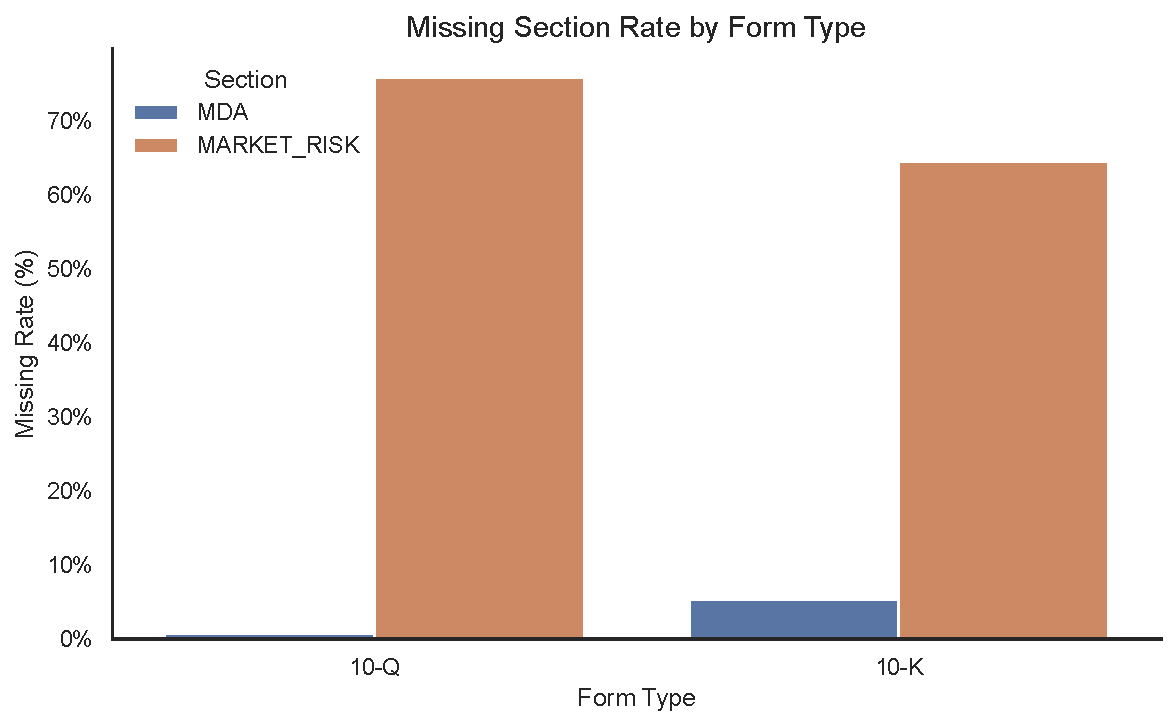
\includegraphics[width=0.75\linewidth]{sec_filings_images/missing_rate_by_form_type.pdf}
    \caption{Missing rate of MD\&A and Market Risk sections by form type (10-K and 10-Q).}
    \label{fig:missing_by_form}
\end{figure}

\section{Text Length Statistics}
\label{appendix:text_length_statistics}

We next examine the statistical properties of the extracted sections based on character count. Observations with zero-length text were excluded from this analysis, as they correspond to missing extractions rather than valid textual content.

The MD\&A section is substantially longer and more variable than the Market Risk section.
While the median filing contains approximately 35,000 characters, the upper tail extends beyond 200,000 characters, reflecting considerable heterogeneity in disclosure practices.
Although the Market Risk section is shorter on average, it also exhibits right-skewness, with a small number of filings containing extensive risk disclosures.

To visualize the distribution of text lengths, we employ a logarithmic scale. This is necessary because SEC filings exhibit heavy-tailed behavior: a small number of extremely long filings would compress the majority of observations near zero on a linear scale. A logarithmic transformation provides a clearer representation of the underlying distributional shape and dispersion.
Filings with zero-length sections were excluded from these plots, as they represent missing extractions rather than valid text.

\begin{figure}[H]
    \centering
    \begin{minipage}{0.48\linewidth}
        \centering
        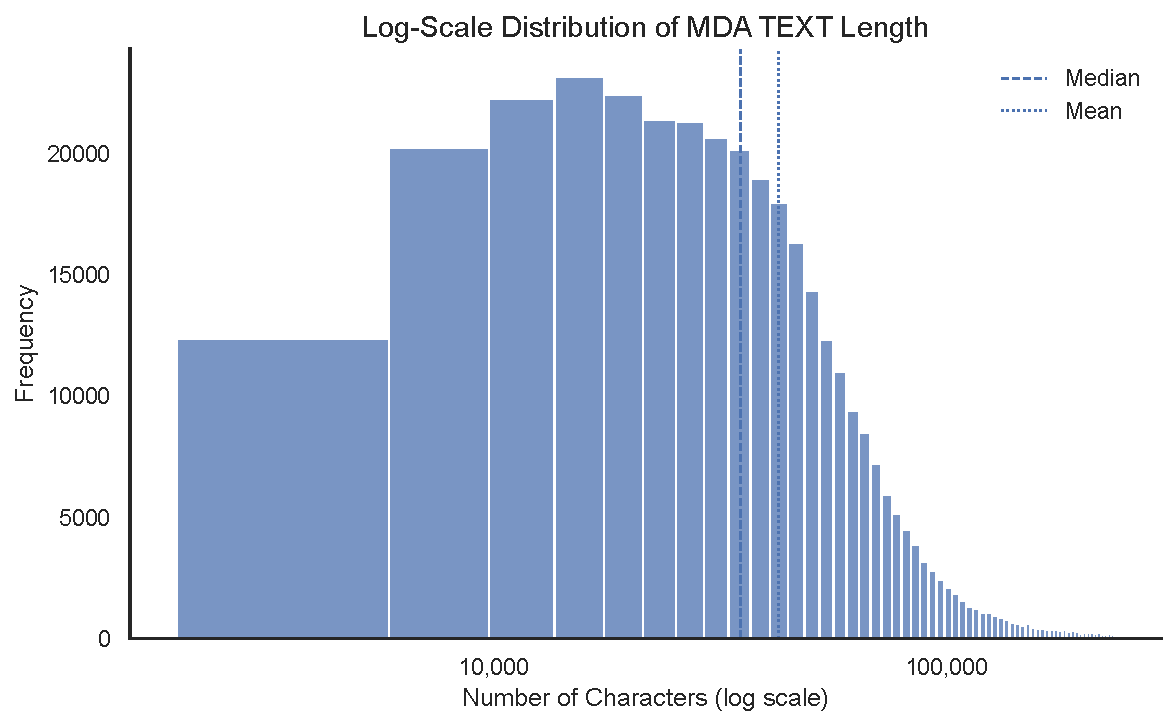
\includegraphics[width=\linewidth]{sec_filings_images/mda_text_length_distribution_log.pdf}
        \caption*{(a) MD\&A}
    \end{minipage}
    \hfill
    \begin{minipage}{0.48\linewidth}
        \centering
        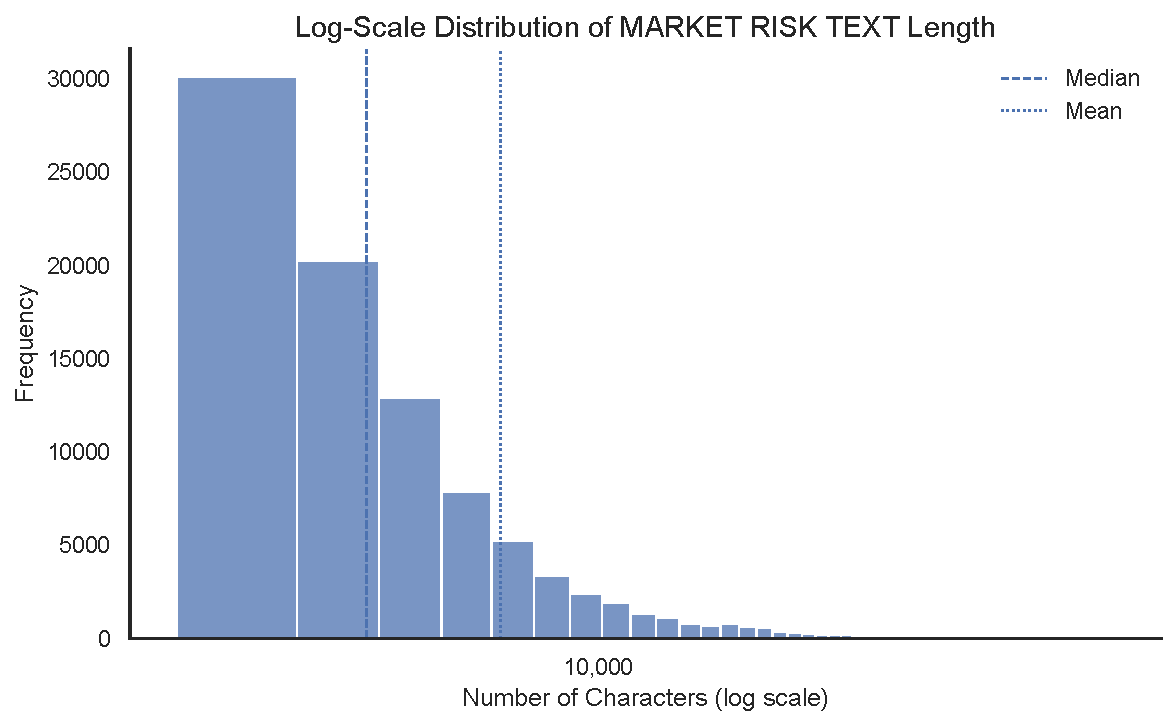
\includegraphics[width=\linewidth]{sec_filings_images/market_risk_text_length_distribution_log.pdf}
        \caption*{(b) Market Risk}
    \end{minipage}
    \caption{Log-scale distribution of section lengths (character count).}
    \label{fig:length_distributions}
\end{figure}

Finally, we examine the temporal distribution of filings. The number of SEC filings per year remains relatively stable throughout the sample period. The highest number of filings occurs in 2011, followed by a gradual and moderate decline toward 2024. The overall stability suggests that the dataset does not suffer from severe temporal imbalance, which is important for downstream modeling tasks.

\begin{figure}[H]
    \centering
    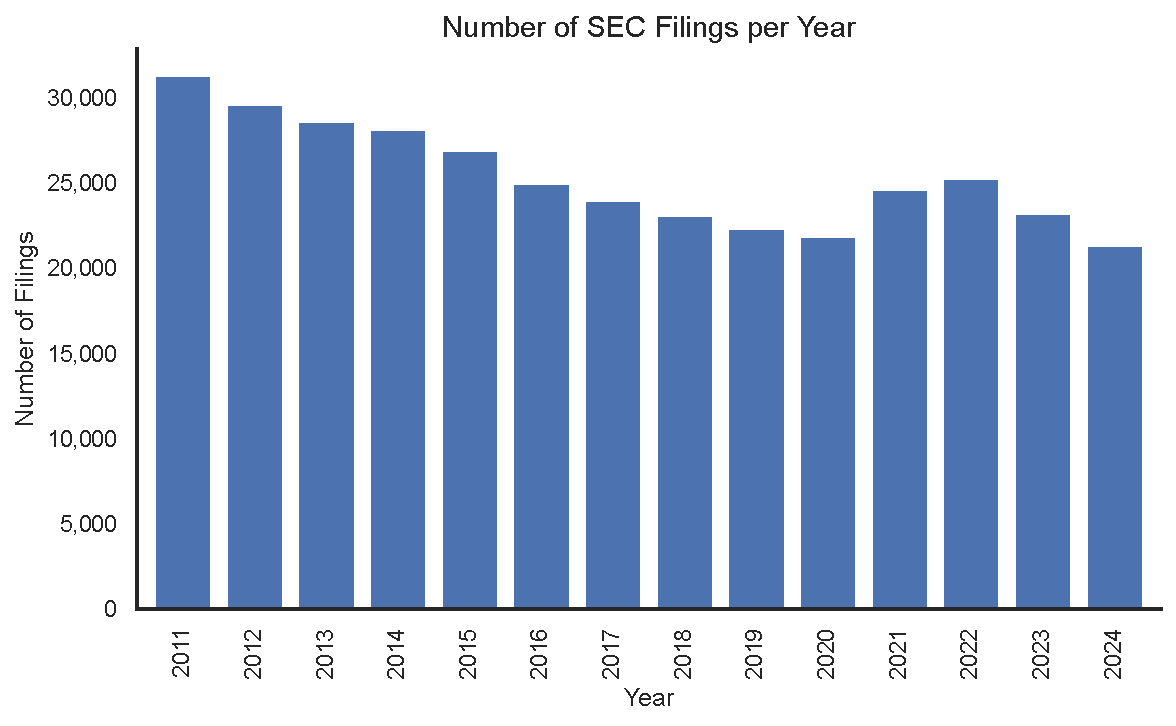
\includegraphics[width=0.75\linewidth]{sec_filings_images/filings_per_year_distribution.pdf}
    \caption{Number of SEC filings per year.}
    \label{fig:filings_per_year}
\end{figure}

Overall, the exploratory analysis confirms that the extraction procedure yields economically meaningful text, that missingness is concentrated primarily in the Market Risk section, and that text length distributions are heavy-tailed and highly heterogeneous. These properties motivate the modeling choices described in subsequent sections, particularly the use of chunk-based processing strategies for long-document sentiment extraction.

\section{Distribution of Filings per Company}
\label{appendix:filings_per_company}

Table-level statistics reveal a moderately dispersed distribution of filings per firm.
The median (33) is very close to the mean (32.58), suggesting that the distribution is not heavily skewed. The 10th percentile indicates that even relatively inactive firms contribute multiple filings (at least six), while firms in the upper quartile contribute more than 54 filings. The maximum of 112 filings suggests that some firms are observed across nearly the entire sample period and across multiple filing types.

Figure~\ref{fig:filings_per_company} visualizes the distribution of filings per firm on a logarithmic scale. The log transformation improves interpretability by preventing firms with very high filing counts from visually compressing the majority of observations.

\begin{figure}[H]
    \centering
    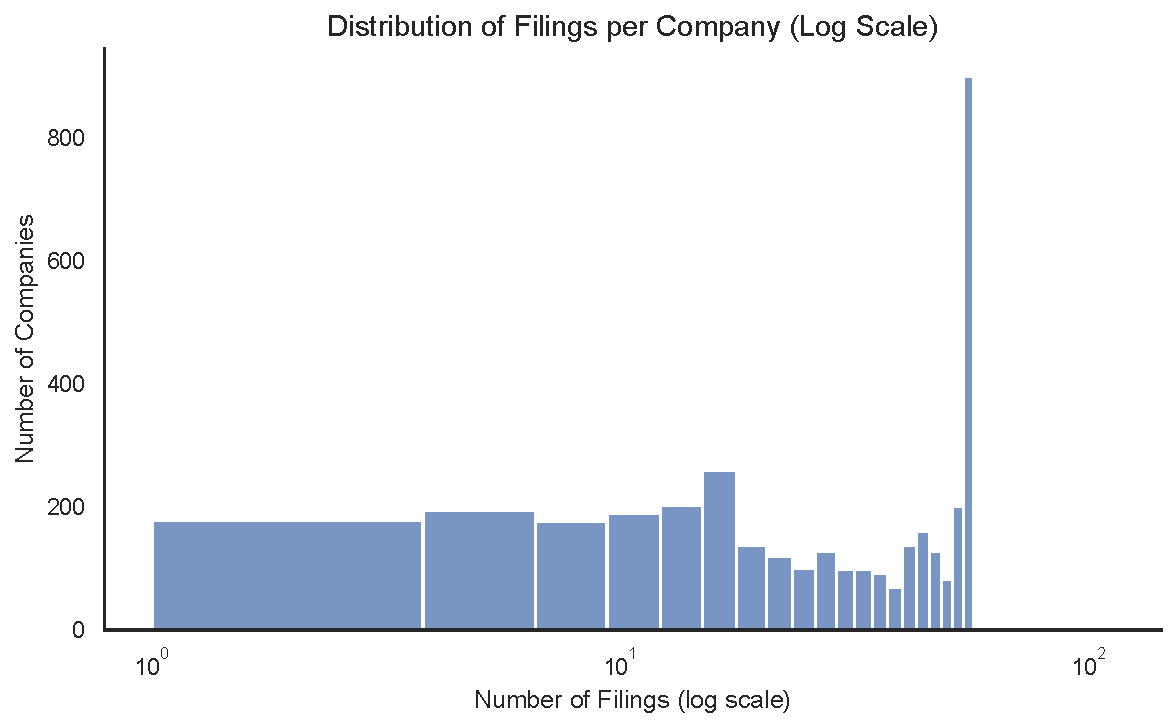
\includegraphics[width=0.75\linewidth]{sec_filings_images/filings_per_company_distribution_log.pdf}
    \caption{Distribution of filings per company (log scale).}
    \label{fig:filings_per_company}
\end{figure}

Overall, the distribution suggests moderate heterogeneity but no extreme dominance by a small number of firms.

\subsection*{Concentration Analysis}

To formally assess whether the dataset is dominated by a small number of highly active firms, we compute filing concentration measures:

\begin{itemize}
    \item Top 1 company share: 0.09\%
    \item Top 5 companies share: 0.39\%
    \item Top 10 companies share: 0.68\%
\end{itemize}

These values indicate very low concentration. Even the ten most active firms together account for less than 1\% of total filings. This is an important property for machine learning applications: the training data is not disproportionately influenced by a handful of firms. Consequently, learned representations are less likely to be biased toward firm-specific disclosure styles of a few dominant entities.

From a statistical perspective, this reduces the risk of overfitting to idiosyncratic firm language patterns and improves the external validity of the trained models.

\subsection*{Time Coverage per Company}

Next, we examine the longitudinal coverage of firms. The median firm is observed for 9.25 years, while firms in the 90th percentile are observed for 13.71 years. The maximum coverage is 13.96 years, which is nearly the full sample period.

Figure~\ref{fig:company_time_coverage} shows the distribution of years covered per firm.

\begin{figure}[H]
    \centering
    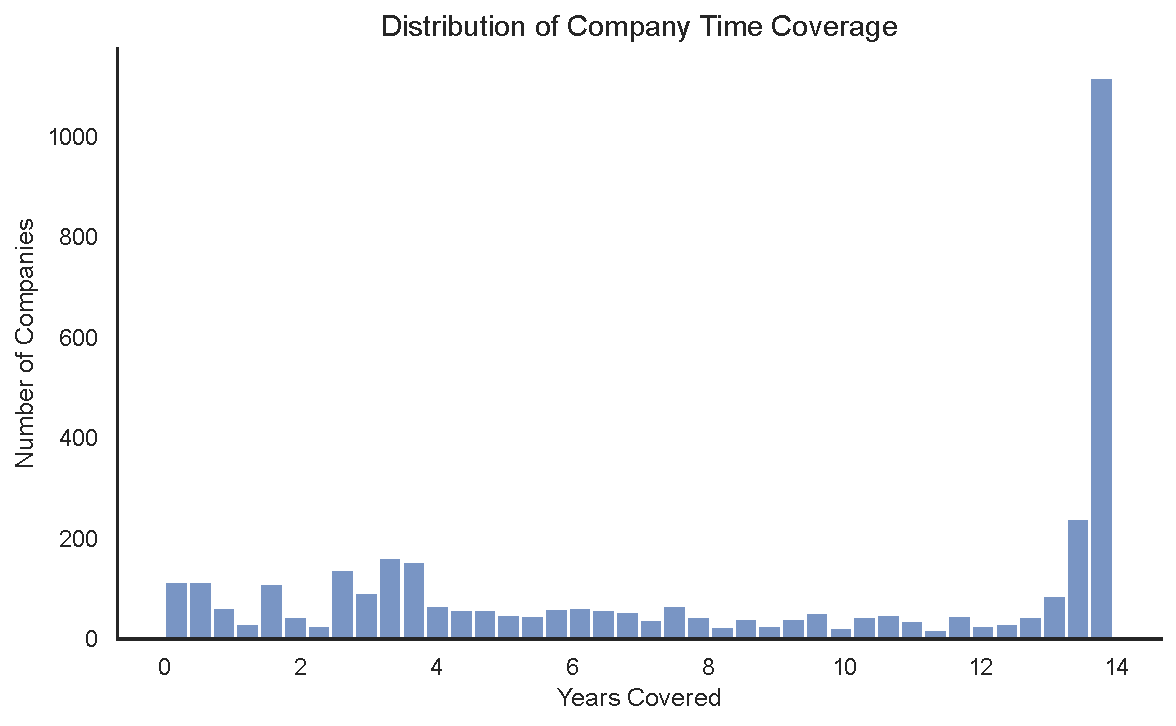
\includegraphics[width=0.75\linewidth]{sec_filings_images/company_time_coverage_distribution.pdf}
    \caption{Distribution of firm time coverage (years).}
    \label{fig:company_time_coverage}
\end{figure}

These statistics indicate that the dataset contains substantial longitudinal depth. Many firms are observed for nearly the entire sample window, while others appear for shorter periods. This structure is typical for financial panel datasets due to IPOs, delistings, mergers, and bankruptcies.

\subsection*{Panel Balance}

To evaluate the balance of the panel, we compute the standard deviation of filings per firm (19.38) and the coefficient of variation (0.59). A coefficient of variation below one indicates moderate dispersion relative to the mean.

This suggests that while firms differ in activity levels, the dataset is not extremely unbalanced. In other words, the panel is heterogeneous but not dominated by a small subset of firms with disproportionately high filing counts.

\subsection*{Implications for Downstream Modeling}

The firm-level analysis highlights several important properties of the dataset:

\begin{enumerate}
    \item \textbf{Strong cross-sectional coverage}: 3,671 firms provide a broad representation of public companies.
    \item \textbf{Meaningful longitudinal depth}: The median firm is observed for over nine years.
    \item \textbf{Low concentration}: Filing activity is not dominated by a small group of firms.
    \item \textbf{Moderate panel imbalance}: Dispersion exists but is not extreme.
\end{enumerate}

Together, these characteristics indicate that the dataset is well-suited for machine learning applications in financial text analysis. It combines sufficient firm diversity with temporal continuity, while avoiding excessive concentration that could distort model training.

\section{Distribution of Sentiment Features}
\label{appendix:sentiment_features}

The results show that the predominant sentiment expressed in the reports is neutral. In particular, 
the median filing exhibits a mean neutral sentiment score above $0.8$, indicating that most sentences 
in financial disclosures are classified as neutral by the model. This observation is consistent with 
the formal and informational tone typically used in financial reporting, where companies tend to 
avoid strongly positive or negative language.

The dispersion of the sentiment scores also reveals notable patterns. The standard deviation of the 
neutral sentiment scores is often larger than that of the positive and negative scores, suggesting 
that while neutral sentiment dominates overall, the degree of neutrality varies more substantially 
across sentences within a filing. In practice, this implies that many reports contain a mixture of 
neutral statements alongside smaller portions of more opinionated or sentiment-bearing language.

Finally, the distribution of the polarity standard deviation exhibits two prominent regions, with 
many filings having values close to $0$ and another concentration around approximately $0.4$. 
Low polarity variability indicates filings in which the sentiment remains highly consistent 
throughout the document, typically reflecting uniformly neutral language. In contrast, higher 
polarity variability suggests documents where sentiment fluctuates more strongly across sections, 
potentially reflecting the coexistence of positive and negative discussions, such as descriptions 
of risks alongside favorable performance indicators.

\begin{figure}
\centering
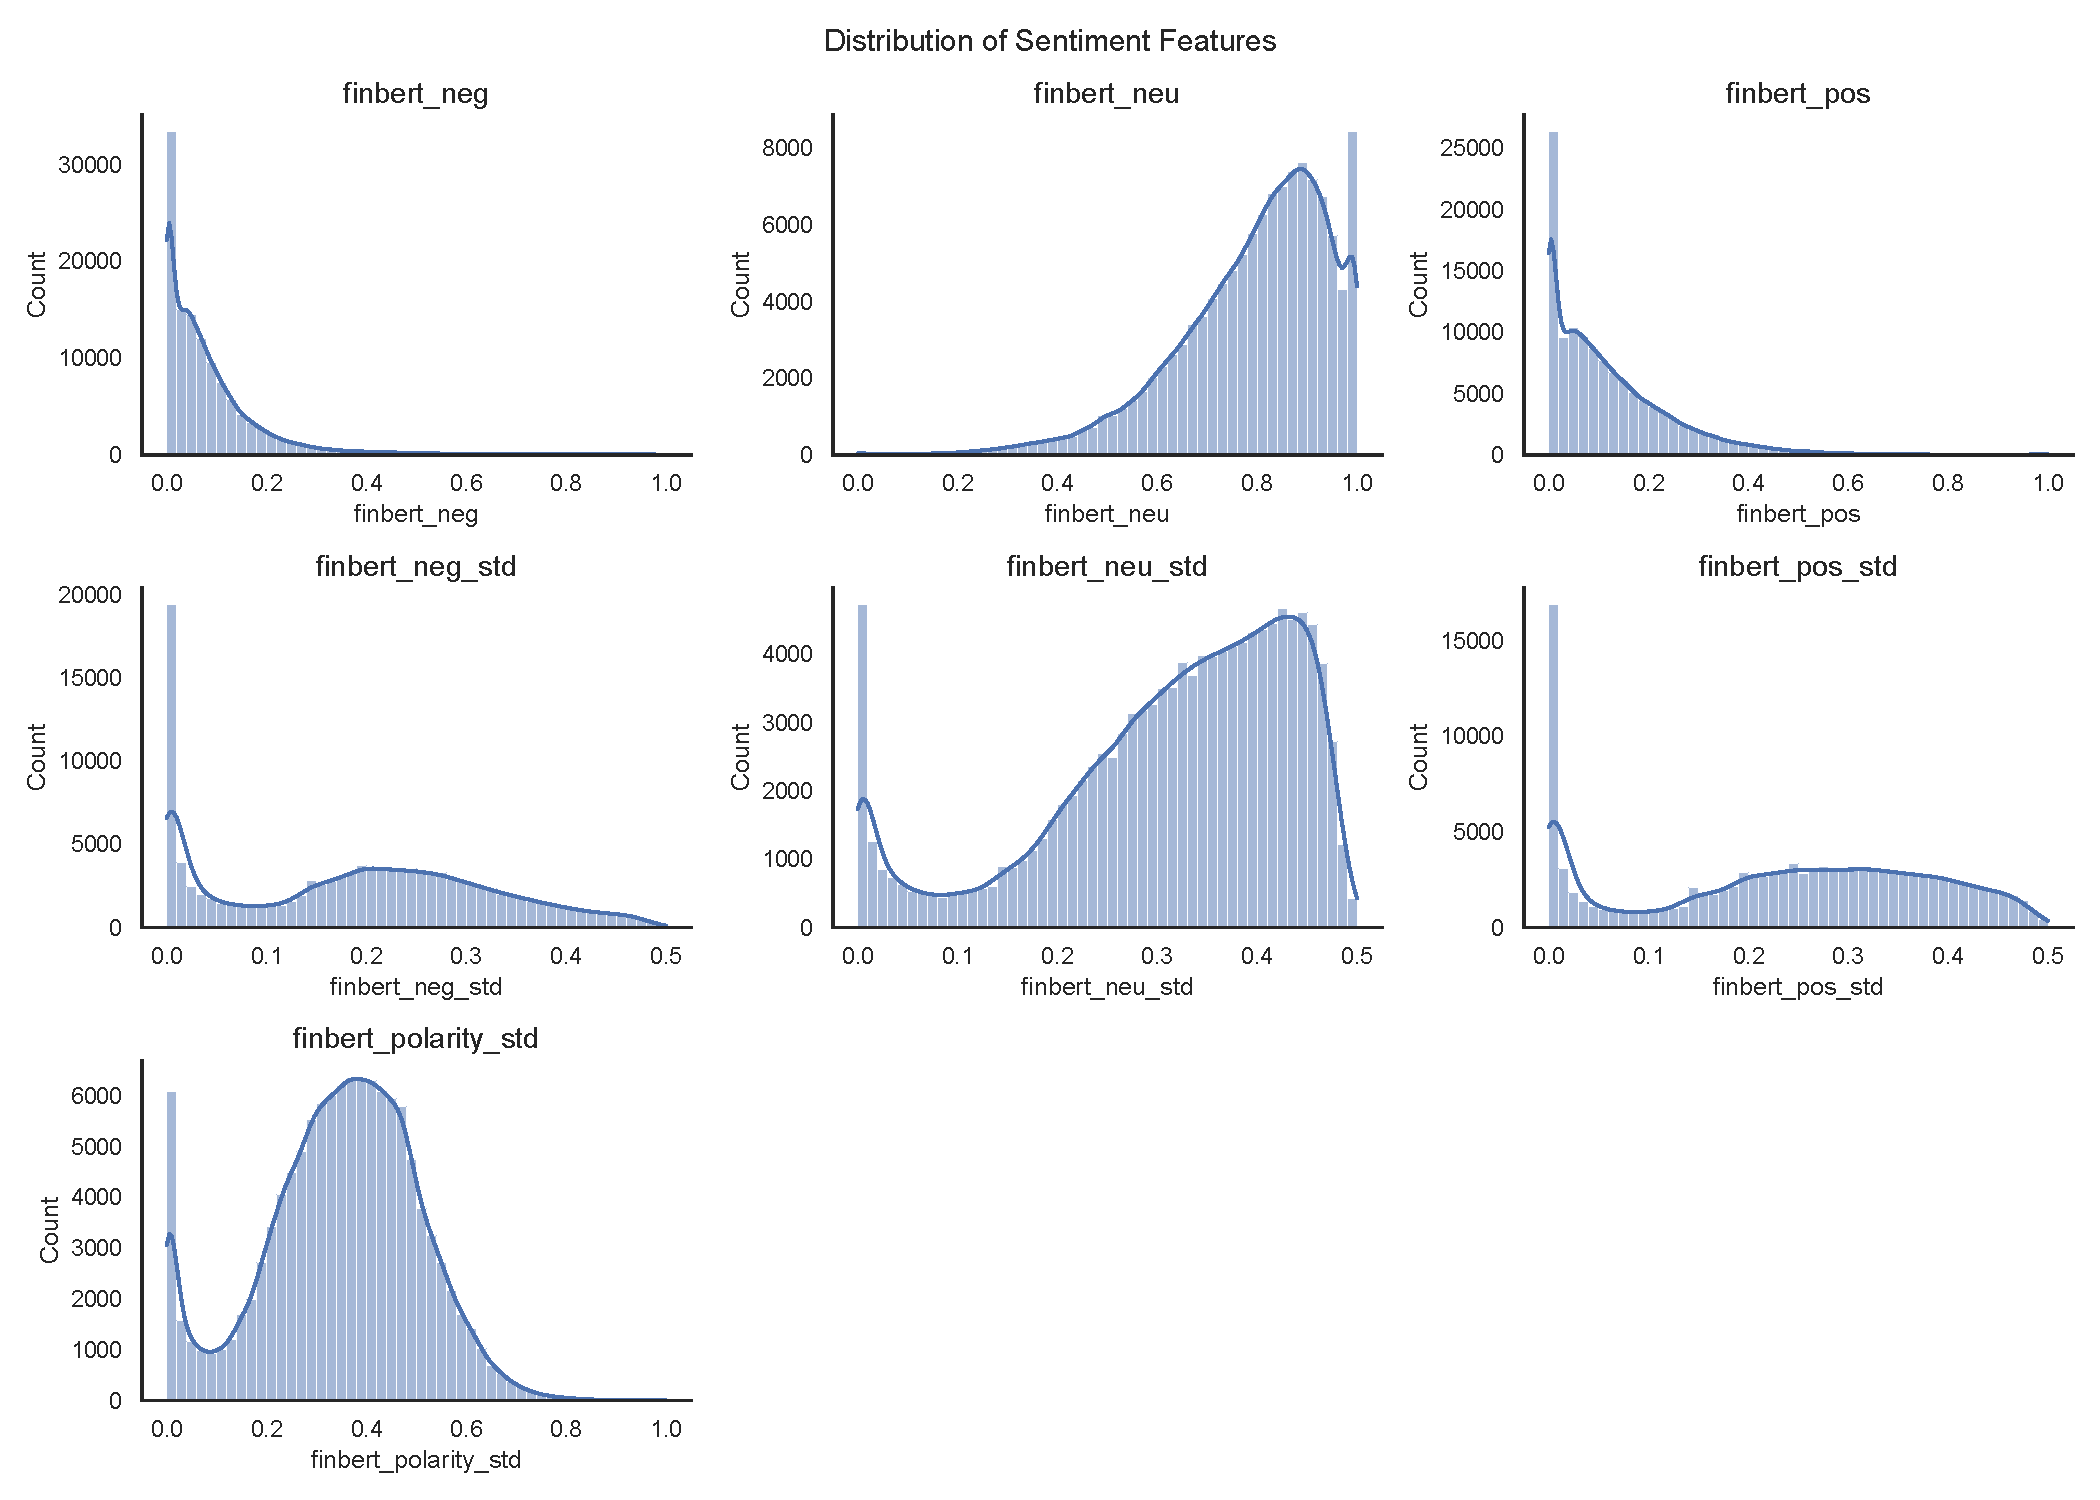
\includegraphics[width=0.9\textwidth]{sec_filings_images/sentiment_scores_distributions.pdf}
\caption{Distribution of the sentiment features extracted from financial filings using the FinBERT model.}
\label{fig:sentiment_distribution}
\end{figure}

\subsection{Sentiment-Gain Delta Distribution}

\begin{figure}
\centering

% ----- Classification Row -----
\begin{subfigure}{0.32\textwidth}
    \centering
    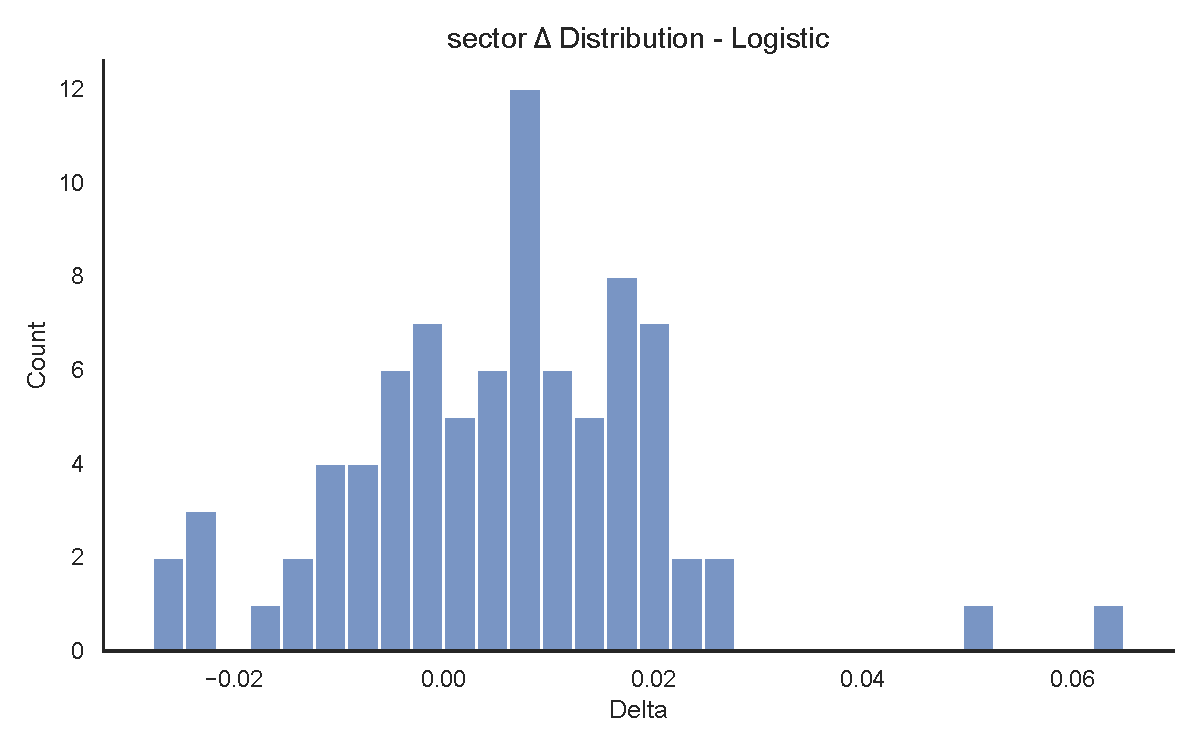
\includegraphics[width=\linewidth]{sector_grouping_comparison_images/sector_classification_delta_distribution_Logistic.pdf}
    \caption{Logistic}
\end{subfigure}
\hfill
\begin{subfigure}{0.32\textwidth}
    \centering
    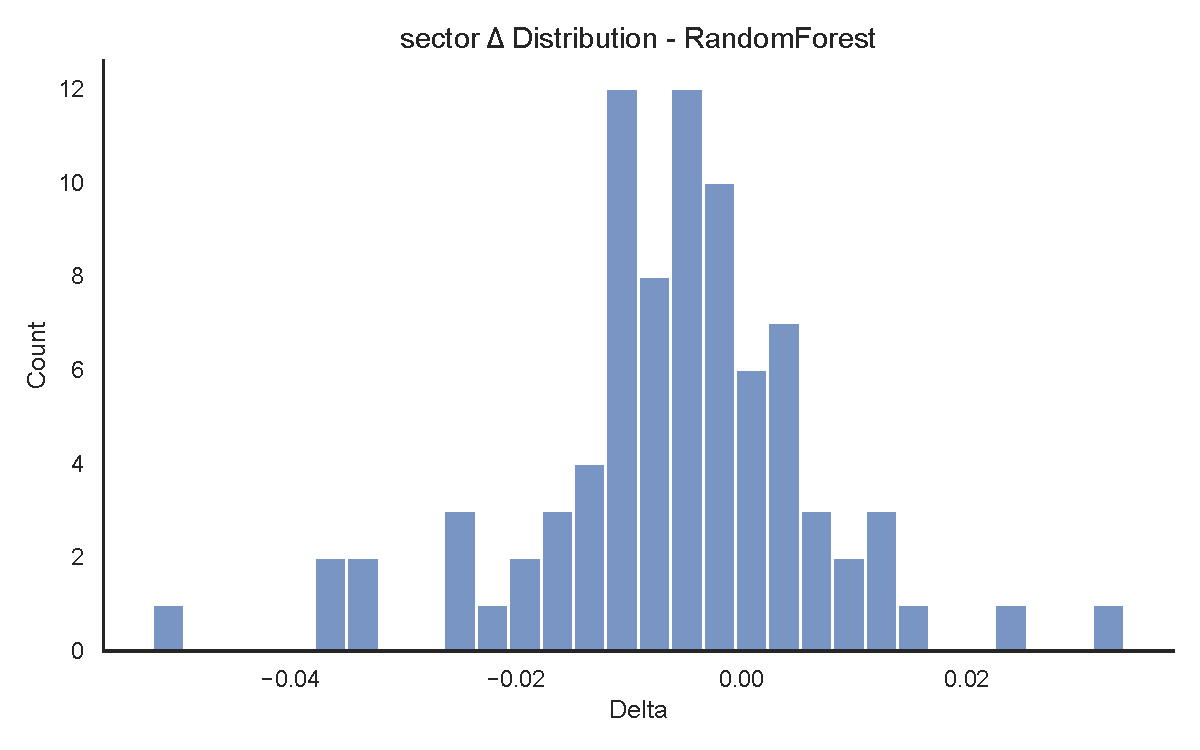
\includegraphics[width=\linewidth]{sector_grouping_comparison_images/sector_classification_delta_distribution_RandomForest.pdf}
    \caption{Random Forest}
\end{subfigure}
\hfill
\begin{subfigure}{0.32\textwidth}
    \centering
    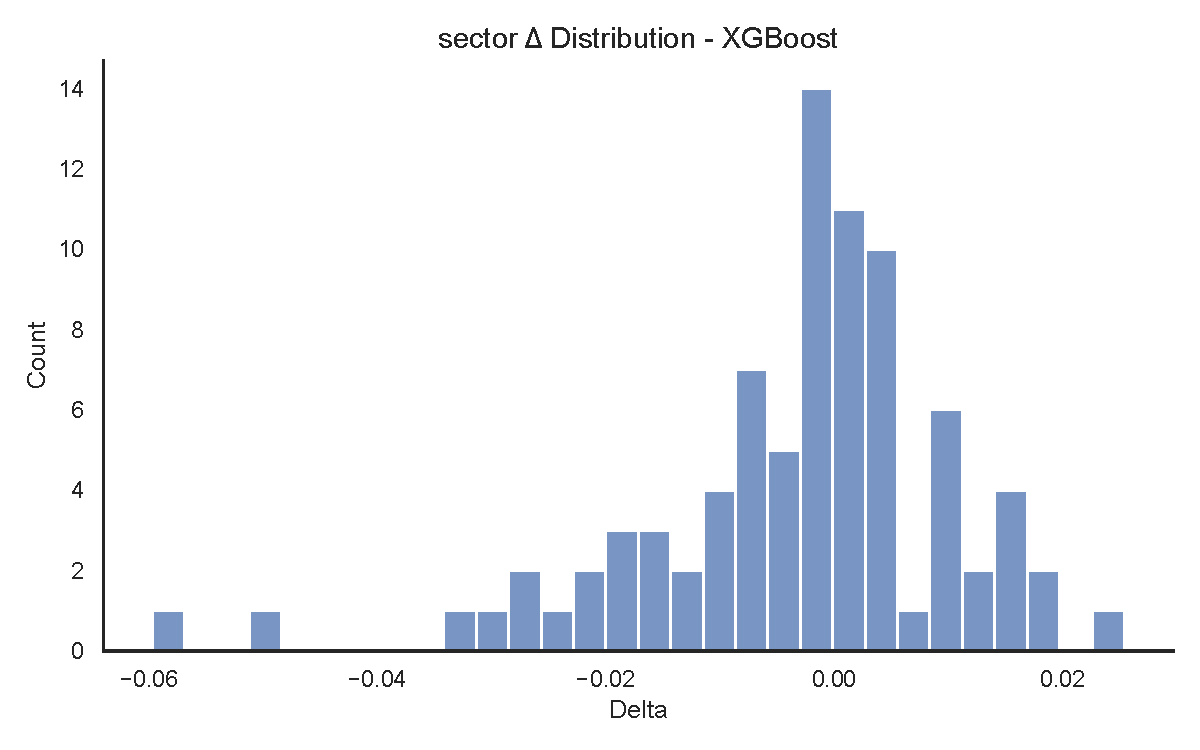
\includegraphics[width=\linewidth]{sector_grouping_comparison_images/sector_classification_delta_distribution_XGBoost.pdf}
    \caption{XGBoost}
\end{subfigure}

\vspace{0.35cm}

\textit{Classification}

\vspace{0.35cm}

% ----- Regression Row -----
\begin{subfigure}{0.32\textwidth}
    \centering
    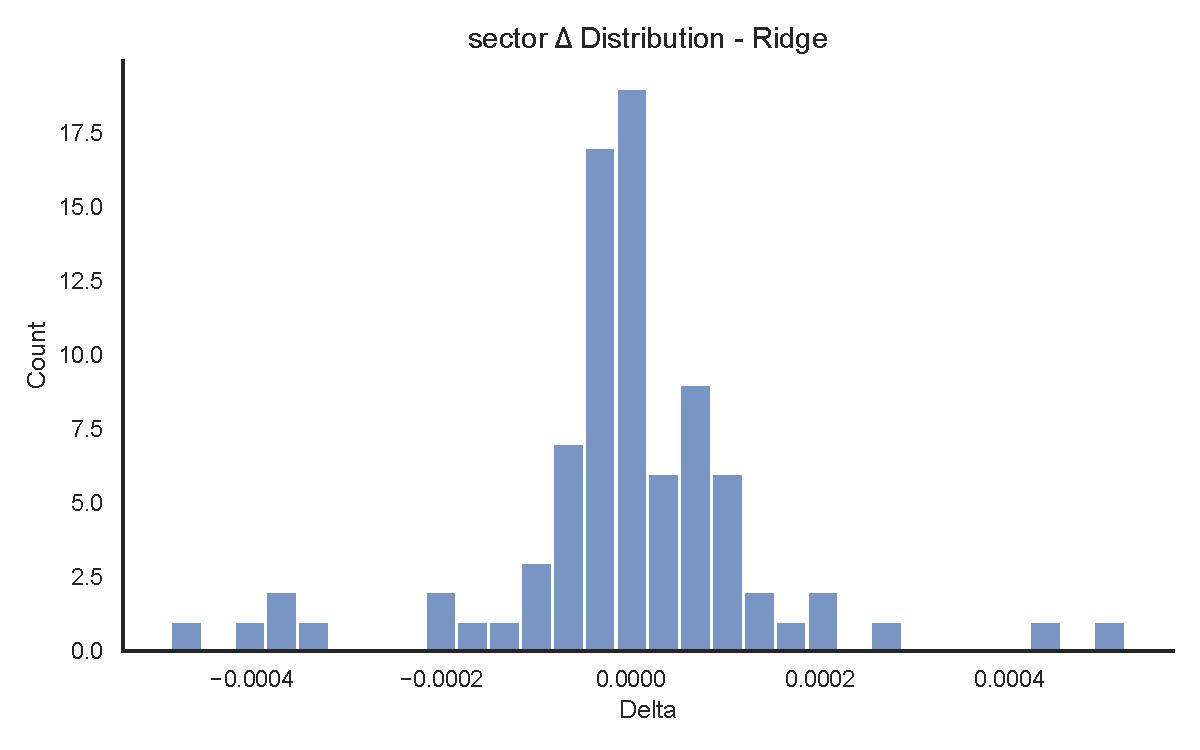
\includegraphics[width=\linewidth]{sector_grouping_comparison_images/sector_regression_delta_distribution_Ridge.pdf}
    \caption{Ridge}
\end{subfigure}
\hfill
\begin{subfigure}{0.32\textwidth}
    \centering
    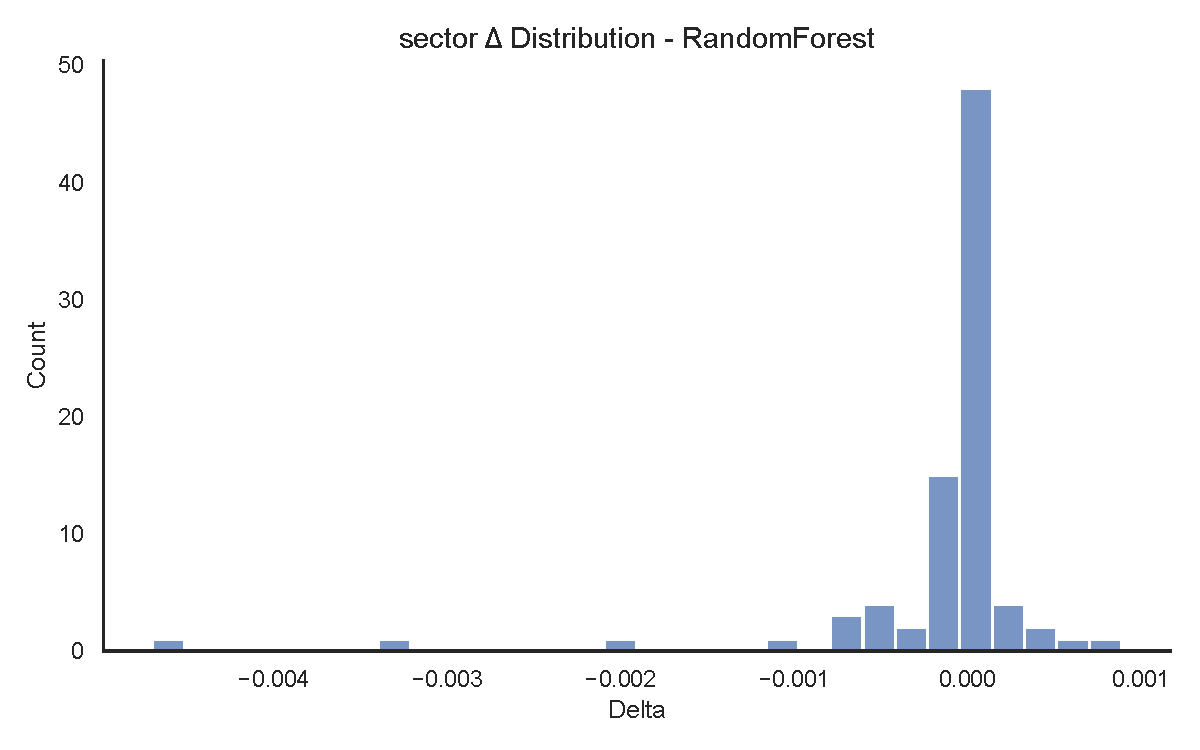
\includegraphics[width=\linewidth]{sector_grouping_comparison_images/sector_regression_delta_distribution_RandomForest.pdf}
    \caption{Random Forest}
\end{subfigure}
\hfill
\begin{subfigure}{0.32\textwidth}
    \centering
    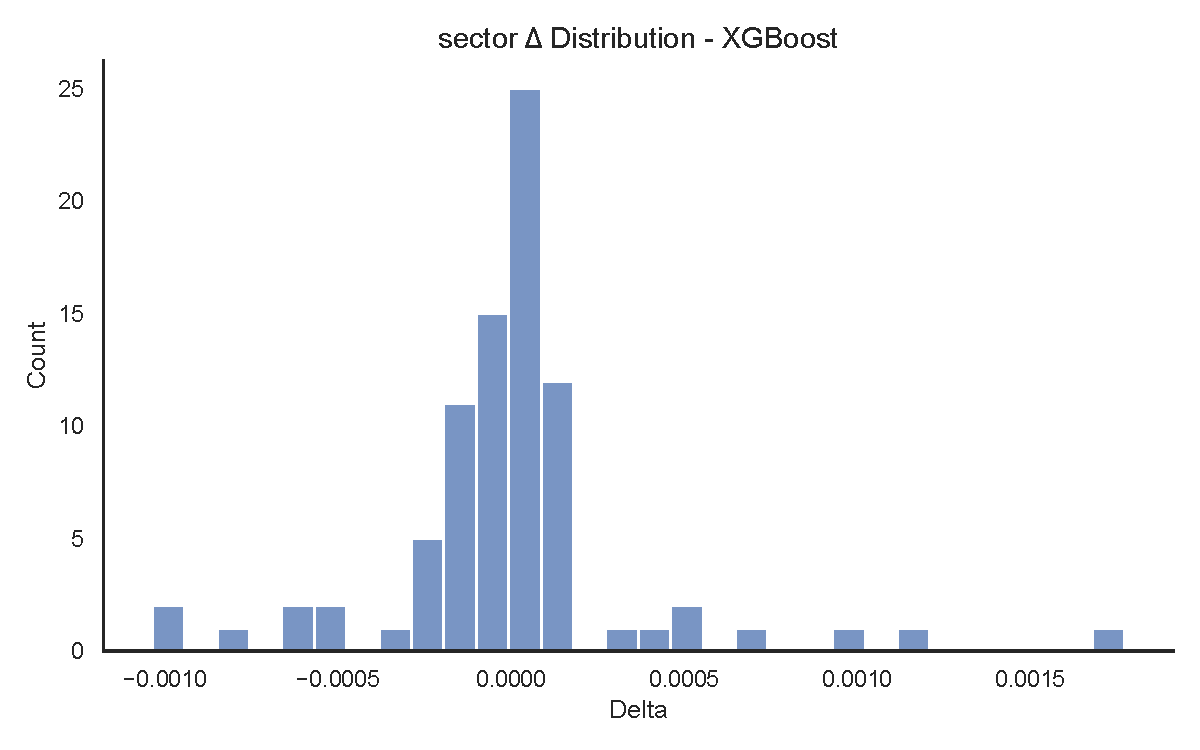
\includegraphics[width=\linewidth]{sector_grouping_comparison_images/sector_regression_delta_distribution_XGBoost.pdf}
    \caption{XGBoost}
\end{subfigure}

\vspace{0.35cm}

\textit{Regression}

\caption{Distribution of performance differences $\Delta$ between models trained with and without sentiment features for the sector-level experiments. Each histogram aggregates $\Delta$ values across all sectors and prediction horizons (1--7 days). The data is mostly concentrated around zero for regression, indicating negligible impact of sentiment features, while classification exhibits a wider spread with noticeable improvements for Logistic regression.}
\label{fig:sector_delta_distribution}
\end{figure}


\begin{figure}
\centering

% ----- Classification Row -----
\begin{subfigure}{0.32\textwidth}
    \centering
    
\includegraphics[width=\linewidth]{sector_grouping_comparison_images/industry_classification_delta_distribution_Logistic.pdf}
    \caption{Logistic}
\end{subfigure}
\hfill
\begin{subfigure}{0.32\textwidth}
    \centering
    
\includegraphics[width=\linewidth]{sector_grouping_comparison_images/industry_classification_delta_distribution_RandomForest.pdf}
    \caption{Random Forest}
\end{subfigure}
\hfill
\begin{subfigure}{0.32\textwidth}
    \centering
    
\includegraphics[width=\linewidth]{sector_grouping_comparison_images/industry_classification_delta_distribution_XGBoost.pdf}
    \caption{XGBoost}
\end{subfigure}

\vspace{0.35cm}

\textit{Classification}

\vspace{0.35cm}

% ----- Regression Row -----
\begin{subfigure}{0.32\textwidth}
    \centering
    
\includegraphics[width=\linewidth]{sector_grouping_comparison_images/industry_regression_delta_distribution_Ridge.pdf}
    \caption{Ridge}
\end{subfigure}
\hfill
\begin{subfigure}{0.32\textwidth}
    \centering
    
\includegraphics[width=\linewidth]{sector_grouping_comparison_images/industry_regression_delta_distribution_RandomForest.pdf}
    \caption{Random Forest}
\end{subfigure}
\hfill
\begin{subfigure}{0.32\textwidth}
    \centering
    
\includegraphics[width=\linewidth]{sector_grouping_comparison_images/industry_regression_delta_distribution_XGBoost.pdf}
    \caption{XGBoost}
\end{subfigure}

\vspace{0.35cm}

\textit{Regression}

\caption{Distribution of performance differences $\Delta$ between models trained with and without sentiment features for the industry-level experiments. Each histogram aggregates $\Delta$ values across all industries and prediction horizons (1--7 days). The data is mostly concentrated around zero for regression, indicating negligible impact of sentiment features, while classification exhibits a wider spread with noticeable improvements for Logistic regression.}
\label{fig:industry_delta_distribution}
\end{figure}

\begin{figure}
\centering

% ----- Classification Row -----
\begin{subfigure}{0.32\textwidth}
    \centering
    
\includegraphics[width=\linewidth]{sector_grouping_comparison_images/ticker_classification_delta_distribution_Logistic.pdf}
    \caption{Logistic}
\end{subfigure}
\hfill
\begin{subfigure}{0.32\textwidth}
    \centering
    
\includegraphics[width=\linewidth]{sector_grouping_comparison_images/ticker_classification_delta_distribution_RandomForest.pdf}
    \caption{Random Forest}
\end{subfigure}
\hfill
\begin{subfigure}{0.32\textwidth}
    \centering
    
\includegraphics[width=\linewidth]{sector_grouping_comparison_images/ticker_classification_delta_distribution_XGBoost.pdf}
    \caption{XGBoost}
\end{subfigure}

\vspace{0.35cm}

\textit{Classification}

\vspace{0.35cm}

% ----- Regression Row -----
\begin{subfigure}{0.32\textwidth}
    \centering
    
\includegraphics[width=\linewidth]{sector_grouping_comparison_images/ticker_regression_delta_distribution_Ridge.pdf}
    \caption{Ridge}
\end{subfigure}
\hfill
\begin{subfigure}{0.32\textwidth}
    \centering
    
\includegraphics[width=\linewidth]{sector_grouping_comparison_images/ticker_regression_delta_distribution_RandomForest.pdf}
    \caption{Random Forest}
\end{subfigure}
\hfill
\begin{subfigure}{0.32\textwidth}
    \centering
    
\includegraphics[width=\linewidth]{sector_grouping_comparison_images/ticker_regression_delta_distribution_XGBoost.pdf}
    \caption{XGBoost}
\end{subfigure}

\vspace{0.35cm}

\textit{Regression}

\caption{Distribution of performance differences $\Delta$ between models trained with and without sentiment features for the company-level experiments. Each histogram aggregates $\Delta$ values across all companies and prediction horizons (1--7 days). The data exhibits a high degree of variability, due to the limiter number of samples available for each company.}
\label{fig:company_delta_distribution}
\end{figure}

\section{Sector and Industry Distribution}
\label{appendix:sector_industry_distribution}

Figure~\ref{fig:companies_per_sector} visualizes the firm-level sector distribution.

\begin{figure}[H]
    \centering
    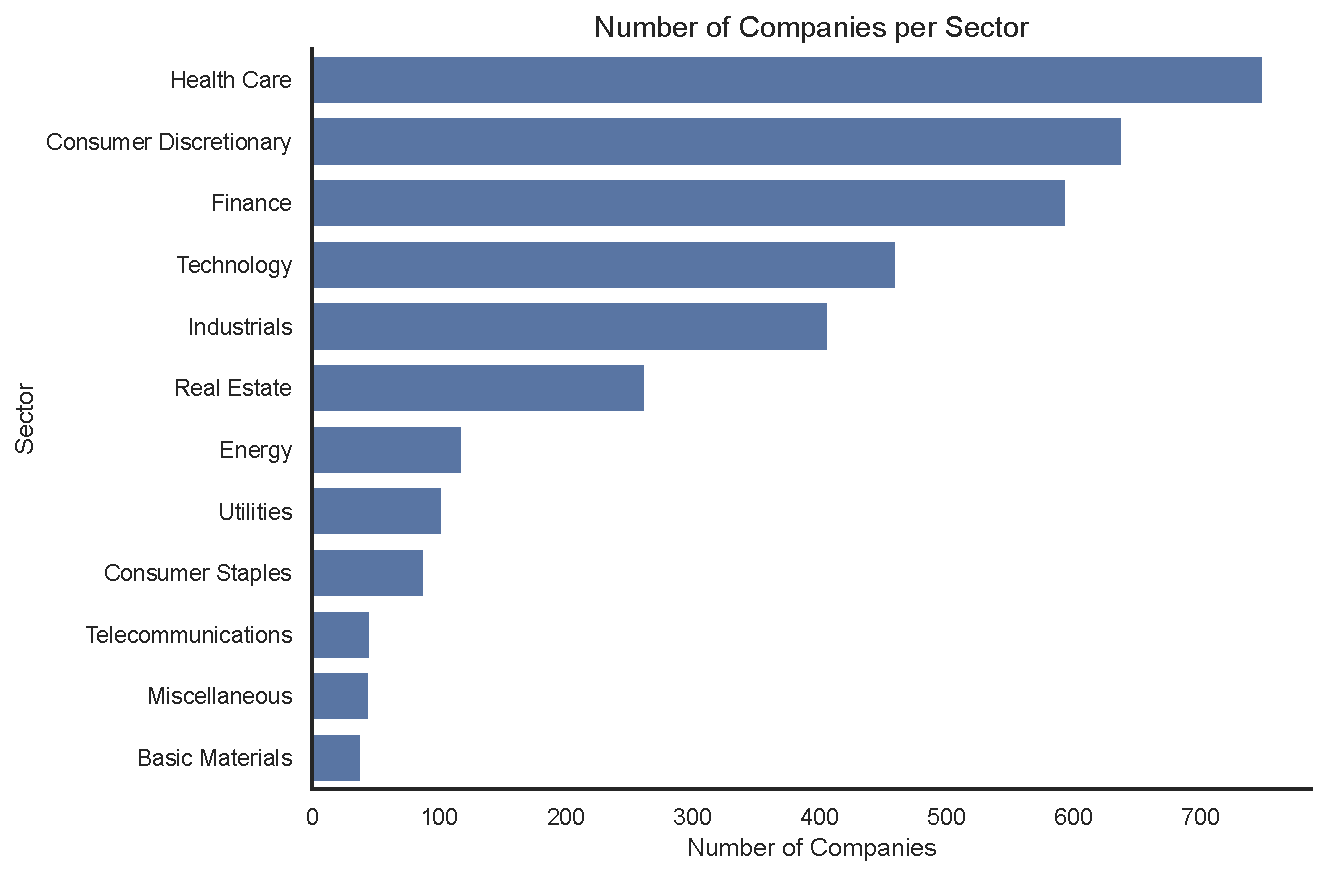
\includegraphics[width=0.8\linewidth]{sec_filings_images/companies_per_sector.pdf}
    \caption{Number of companies per sector.}
    \label{fig:companies_per_sector}
\end{figure}

When examining the distribution at the filing level, slight differences emerge.
The ordering differs somewhat from the firm-level ranking, indicating that certain sectors contribute more filings per firm on average. For example, Consumer Discretionary produces more filings than Health Care despite having fewer firms. This suggests differences in reporting intensity across sectors.

Figure~\ref{fig:filings_per_sector} illustrates the filing-level sector distribution.

\begin{figure}[H]
    \centering
    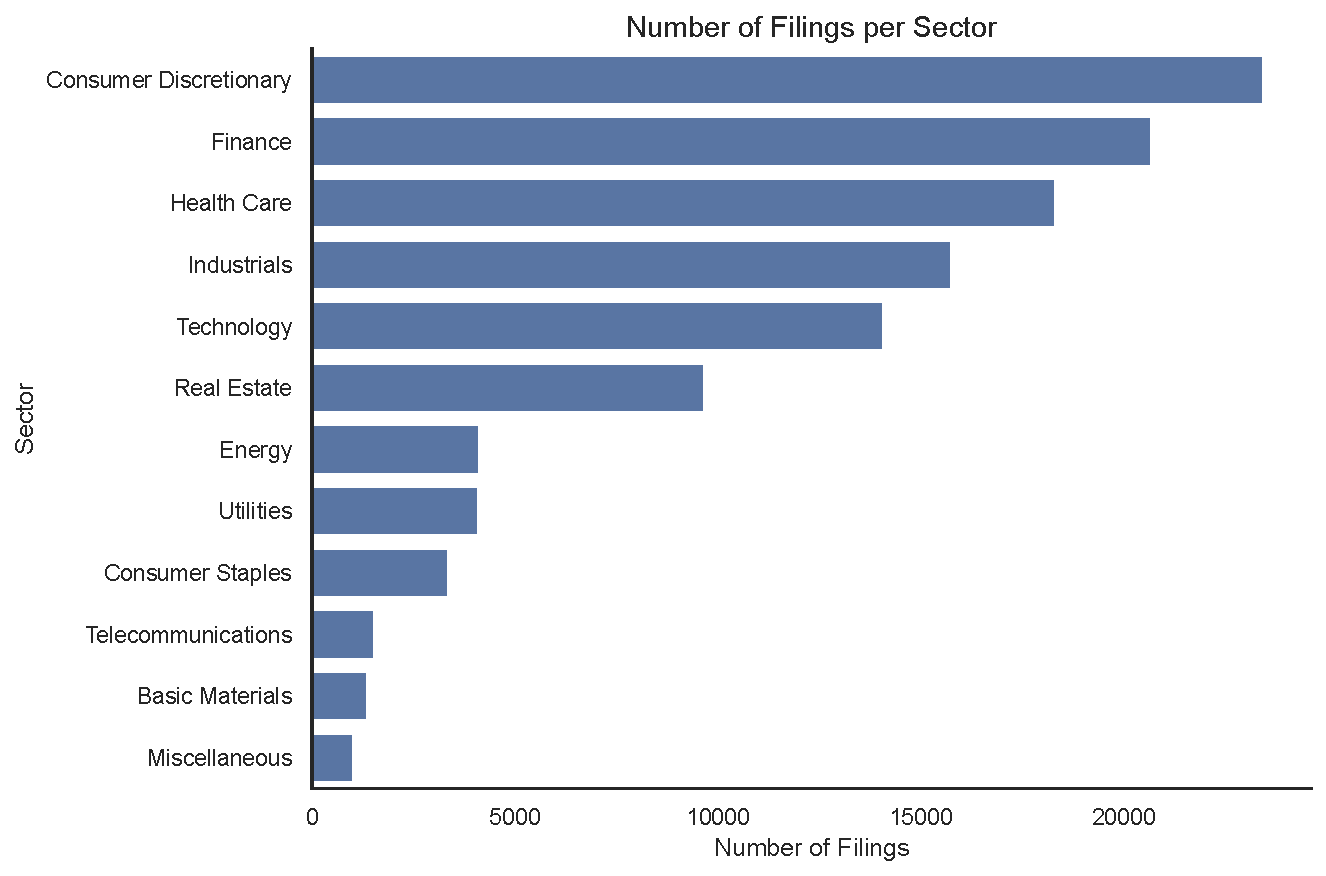
\includegraphics[width=0.8\linewidth]{sec_filings_images/filings_per_sector.pdf}
    \caption{Number of filings per sector.}
    \label{fig:filings_per_sector}
\end{figure}

From a modeling perspective, this distinction is important: sector imbalance at the firm level does not necessarily imply imbalance in the volume of textual training data. Models trained on filings may be more influenced by sectors with higher reporting intensity.

At the industry level, the dataset contains 149 distinct industries, substantially increasing granularity relative to the 12-sector classification.
The dominance of biotechnology-related industries is particularly notable, reflecting the large number of publicly traded pharmaceutical and biotech firms.

However, the overall industry distribution exhibits a pronounced long-tail structure. The median number of companies per industry is 11. While a few industries contain hundreds of firms, many industries are represented by only a handful of companies.

Figure~\ref{fig:top20_industries} displays the top 20 industries by firm count, while Figure~\ref{fig:industry_long_tail} visualizes the full distribution on a logarithmic scale.

\begin{figure}[H]
    \centering
    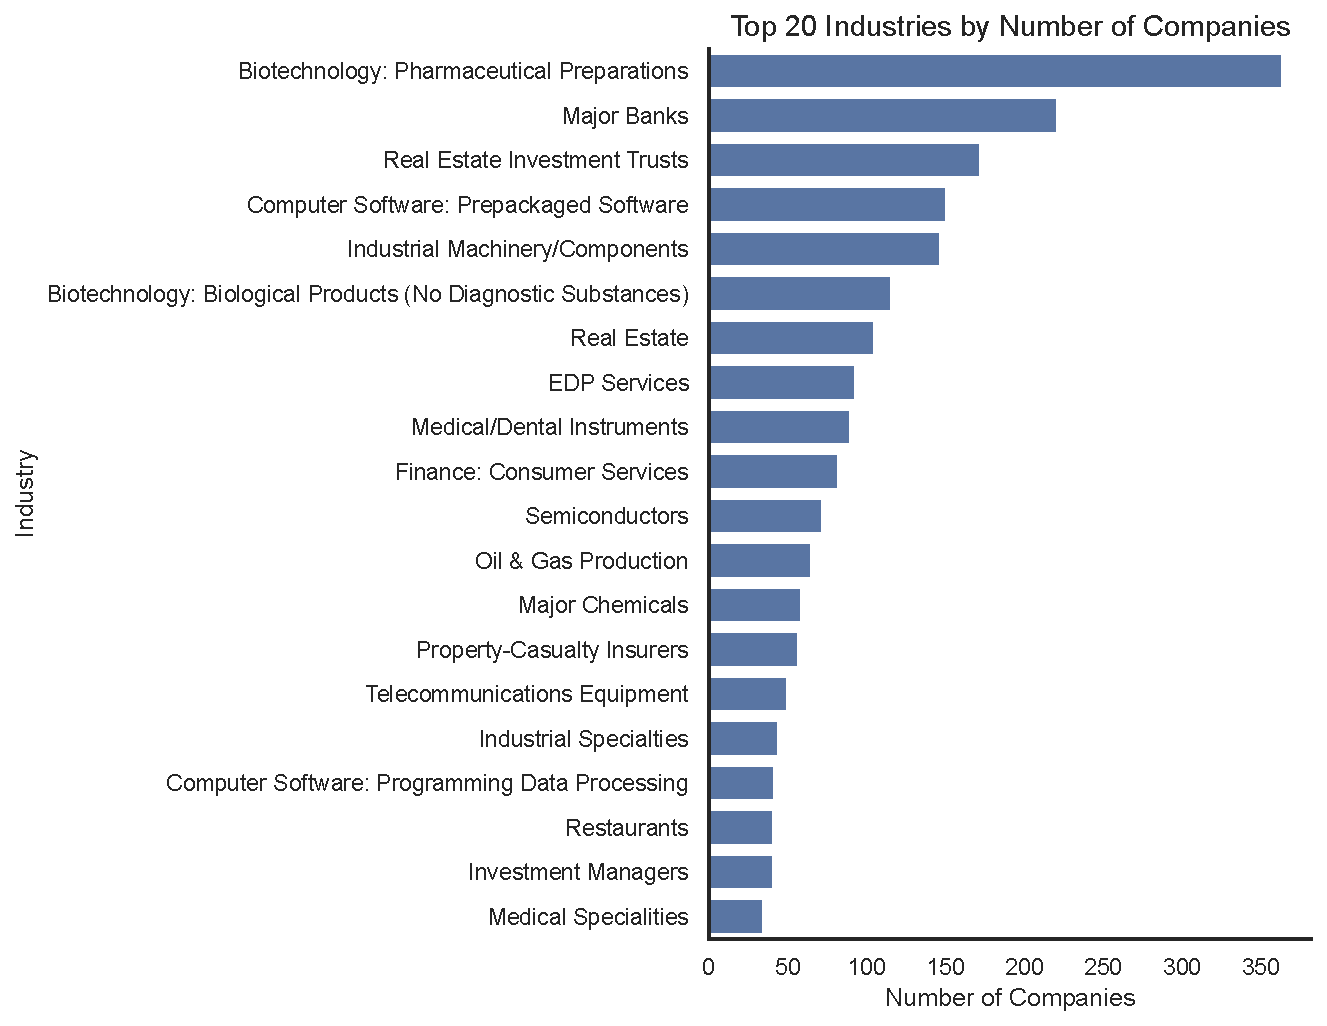
\includegraphics[width=0.85\linewidth]{sec_filings_images/top20_industries_by_companies.pdf}
    \caption{Top 20 industries by number of companies.}
    \label{fig:top20_industries}
\end{figure}

\begin{figure}[H]
    \centering
    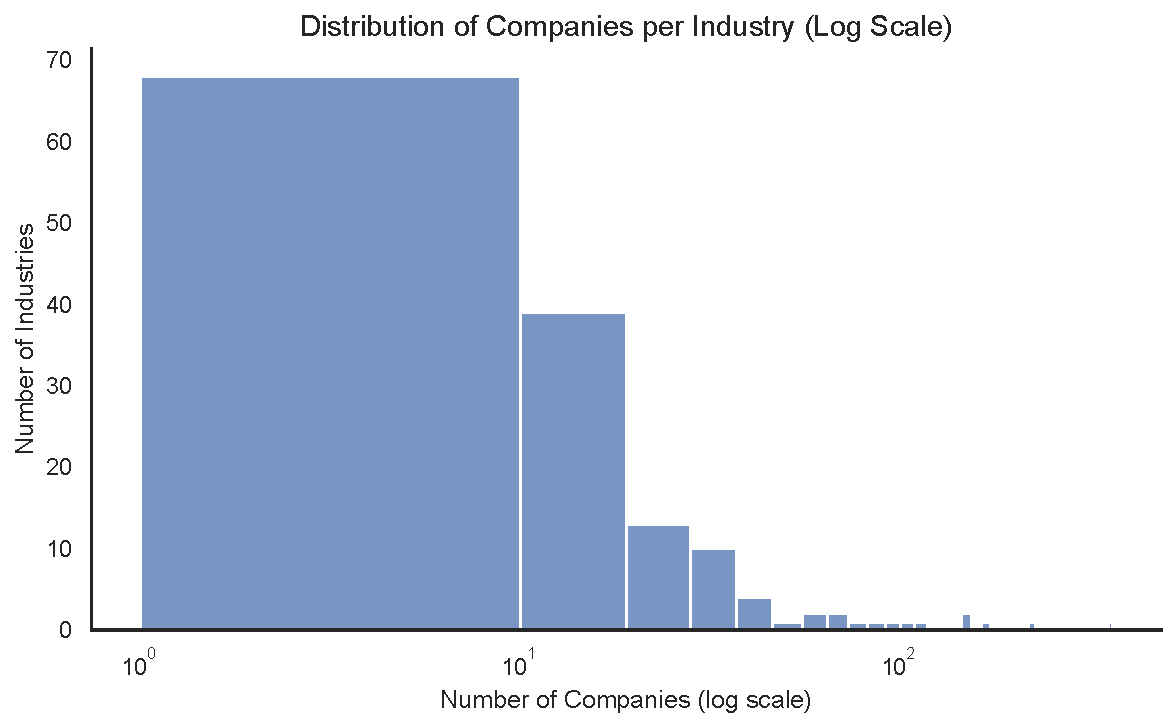
\includegraphics[width=0.75\linewidth]{sec_filings_images/industry_company_distribution_log.pdf}
    \caption{Distribution of companies per industry (log scale).}
    \label{fig:industry_long_tail}
\end{figure}

The logarithmic representation highlights the heavy-tailed nature of industry representation. Many industries contain relatively few firms, while a small number of industries dominate in terms of firm count.

\subsection*{Implications for Modeling}

The sector and industry composition of the dataset has several implications:

\begin{enumerate}
    \item \textbf{Broad economic coverage:} With 12 sectors and 149 industries, the dataset spans a wide range of economic activity.
    \item \textbf{Moderate sector imbalance:} Some sectors (e.g., Health Care, Consumer Discretionary, Finance) contain significantly more firms than others.
    \item \textbf{Industry-level fragmentation:} The industry distribution is highly skewed, with a pronounced long tail.
    \item \textbf{Potential heterogeneity in disclosure style:} Sector- and industry-specific language patterns may influence textual sentiment extraction and predictive performance.
\end{enumerate}